\documentclass[letterpaper]{article}

\usepackage{./qilinnotes}

\newcommand\Class{Grade 12 Bio}
\newcommand\Unit{Biochemistry}
\newcommand\Author{QiLin Xue}

\begin{document}
\maketitle

\tableofcontents
\newpage

\begin{review}
    \textbf{Organization} - New Properties Emerge at Successive Levels of Biological Organization - Hierarchy of Life, Emergent Properties and Systems \\

    We use strategies of \textbf{reductionism} to make the study of biology more manageable - but incomplete. How do the cells work together? By zooming out, we can look at \textbf{emergent} properties. In this unit, we will zoom in even more to look at the processes that make up individual cell parts.
\end{review}
\section{Properties of Water}
\begin{itemize}
    \item Water molecules bond with each other through \textbf{cohesion}, creating a high surface tension. This allows water striders to walk on the surface.
    \begin{itemize}
        \item Chemicals called surfactants can be added to make water lose its surface tension $\gamma$.
    \end{itemize}
    \item Water molecules form hydrogen bonds with other polar molecules through \textbf{adhesion}, allowing capillary action to move water up xylem tubes. This also causes water to dissolve other polar substances.
    \item Hydrogen bonding causes water to absorb large amounts of thermal energy, creating a \textbf{high specific heat capacity} to moderate temperatures.
    \item Strong hydrogen bonding takes a lot of energy to break, resulting in a high specific heat of vaporization creating evaporative cooling effects.
    \item Water forms a \textbf{wide lattice structure} in its solid state, allowing ice to float on water creating an insulation for marin environments during Winter.
\end{itemize}
\newpage
\section{Carbon Chemistry of Life}
\begin{itemize}
    \item The backbone of most organic molecules contain an alkane backbone (e.g. decane):
    \begin{center}\chemfig{
        -[:30]-[:-30]-[:30]-[:-30]-[:30]-[:-30]-[:30]-[:-30]-[:30]
    }\end{center}
    \begin{tip}
        The $n$ number describes the number of carbons in the alkane backbone such that the chemical formula is:
        $$C_nH_{2n+2}$$
        Naming is in the form of \textit{prefix-ane} where the prefix is given by the following chart:
        \begin{multicols}{3}
        \begin{itemize}
            \item Meth (n=1)
            \item Eth (n=2)
            \item Prop (n=3)
            \item But (n=4)
            \item Pent (n=5)
            \item Hex (n=6)
            \item Hept (n=7)
            \item Oct (n=8)
            \item Non (n=9)
        \end{itemize}
        \end{multicols}
        For example, an alkane with five carbons will be known as pentane and have a chemical formula of $C_5H_{12}$.
    \end{tip}
    \subsection{Functional Groups}
    \item Functional groups are specific substituents within molecules that are responsible for the characteristic chemical reactions.
    \item \textit{Alcohols} contain the \textbf{hydroxyl} functional group with the suffix -ol (e.g. ethanol):
    \begin{center}
    % \chemfig{C(-[2]H)(-[4]H)(-[6]H)-C(-[2]H)(-[6]H)-[@{b1,0}]O@{H}H}
    \chemfig{-[:30]-[:-30]OH}
    % \chemmove{
    % \draw[-,red]
    %     (b1) -- ++(0,.25) -| (H.east)
    %     (b1) -- ++(0,-.25) -| (H.east) ;
    % }
    \end{center}

    \item Carboxylic acids have a \textbf{carboxyl group} with the suffix -oic acid (ethanoic acid): \label{sec:carboxylic}
    \begin{center}
        % \chemfig{C(-[2]H)(-[4]H)(-[6]H)-C(=[1]O)(-[7]OH)}
        \chemfig{-[:30](-[:-30]OH)(=[:90]O)}
    \end{center}
    \begin{tip}
    Note, the $n$ number doesn't include the carbon in the carboxyl group such that the general formula is
    $$C_nH_{2n+1}NH_2$$
    However, the nomenclature prefix is based on the total number of carbons.
    \end{tip}
    \item \textit{Amino acids} have an $NH_2$ as their functional group. It has a prefix of "amino-" (e.g. aminomethane):
    \begin{center}
        % \chemfig{C(=[3]O)(-[5]HO)-C(-[2]CH_3)(-[6]H)-N(-[1]H)(-[7]H)}
        % \chemfig{NH_2-[:-30]-[:30](-[:-30]OH)(=[:90]O)}
        \chemfig{R-NH_2}
    \end{center}

    \item \textit{Aldehydes} have a \textbf{carbonyl} group at the end of the molecule (e.g. ethanal):
    \begin{center}
        \chemfig{-[:30]=[:-30]O}
        % \chemfig{H-C(-[2]H)(-[6]H)-C(-[7]H)=[1]O}
    \end{center}
    
    Because oxygen is more electronegative than carbon, it draws electron density away from carbon, increasing the bond's polarity. \textit{This means it is more likely to react.}
    \item The carbonyl group in a \textit{ketone} is connected to two carbons instead of a carbon and an oxygen (e.g. acetone):
    \begin{center}
        % \chemfig{C(-[2]H)(-[4]H)(-[6]H)-C(=[6]O)-C(-[0]H)(-[2]H)(-[6]H)}
        \chemfig{-[:30](=[:90]O)-[:-30]}
    \end{center}
    \item Many cellular molecules also have a \textbf{sulfhydryl}  group (e.g. mercaptoethanol):
    \begin{center}
        \chemfig{
            % C(-[2]H)(-[4]HO)(-[6]H) - 
            % C(-[2]H)(-[6]H)(-[0]SH)
            -SH
        } \\
    \end{center}
    \item \textit{Nucleotides}, nucleic acids, and many other cellular molecules have a \textbf{phosphate} group:
    \begin{center}
        % \chemfig{
            % C(=[3]O)(-[5]H)-
            % C(-[2]H)(-[6]OH)-
            % C(-[2]H)(-[6]H)-
        % }
        \chemfig{
            R-
            O-
            P(-[0]O^{-})(-[2]O^{-})(=[6] O^{-})
        }
    \end{center}
    \subsection{Amino Acids}
    \item Amino acids contain two functional groups, an amine group and a carboxyl group. It also contains one other group of atoms called an R-group
    \begin{center}
        \chemfig{
            N(-[3]H)(-[5]H)-C(-[2]H)(-[6]R)-C(=[1]O)(-[-1]OH)
        }
    \end{center}
    The chemical formula is written as \ce{NH_2CHRCOOH}
    \subsection{Reactions Between Functional Groups}
    \item \textbf{Ether} linkages are formed when two alcohols combine together. They can be identified by looking for the $COC$ link.
    \begin{center}
    \ce{
        \chemfig{H_3COH} +
        \chemfig{HOCH_2CH_3}
        ->
        \chemfig{H_3COCH_2CH_3} + H2O
    }
    \end{center}
    Since a water molecule is being produced, this is known as a \textbf{condensation} reaction. The reverse would be known as a \textbf{hydrolysis} reaction.
    \item \textbf{Ester} linkages are formed when an alcohol and a carboxylic acid combine. They can be identified by looking for the $OCO$ link.
    \begin{center}
        \ce{
            \chemfig{CH_3OH} +
            \chemfig{CH_3COOH}
            ->
            \chemfig{CH_3OCOCH_3} + H2O
        }
    \end{center}
    \item Phosphate ester linkages are formed when an alcohol reacts with a phosphoric acid.
    \begin{center}
        \ce{
            \chemfig{CH_3OH} +
            \chemfig{H_3PO_4}
            ->
            \chemfig{CH_3OPO_3H_2} + H2O
        }
    \end{center}
    \item \textbf{Peptide} linkages form between amino acids where the $OH$ from the carboxyl group combines with the $H$ from the amine group. This allows it to be connected in long chains:
    \begin{center}
        \ce{
            \chemfig{NH_2CH_2COOH} +
            \chemfig{NH_2CH_2COOH}
            ->
            \chemfig{NH_2CH_2CONHCH_2COOH} + H2O
        }
    \end{center}
    \end{itemize}
\newpage
\section{Macromolecules}
    \begin{itemize}
    \item Tiny molecules can create long polymers to form macromolecules with new emergent properties that come from its building blocks. THese are the building blocks of organelles.
    \begin{idea}
        Polymers are made from different monomers. Here are the monomers for the main four macromolecules:
        \begin{multicols}{2}
        \begin{itemize}
            \item Carbohydrates (Sugars)
            \item Lipids (Fatty Acids)
            \item Proteins (Amino Acids)
            \item Nucleic Acids (Nucleotides)
        \end{itemize}
        \end{multicols}
    \end{idea}
    \subsection{Carbohydrates}
    \item Carbohydrates generally contain CHO atoms in a 1:2:1 ratio and is recognized by the "ose" ending. They are either simple or complex and can undergo dehydration reactions.
    \begin{itemize}
        \item The three main purposes: \textit{energy source, structural component, cell-cell communication}
    \end{itemize}
    \item One type of simple carbs are \textbf{Monosaccharides} (\textit{mono- = “one”; sacchar- = “sugar”}) are simple sugars with the chemical formula of \ce{(CH_2)_n}. Most of the oxygen atoms in monosaccharides are found in hydroxyl groups, but one of them is part of a carbonyl group. 
    \item \textit{Glucose} is a common sugar (blood sugar) that turns into a ring shape when put in solution. The difference between the $\alpha$ glucose and the $\beta$ glucose is in the orientation of the \ce{OH} group.
    \begin{center}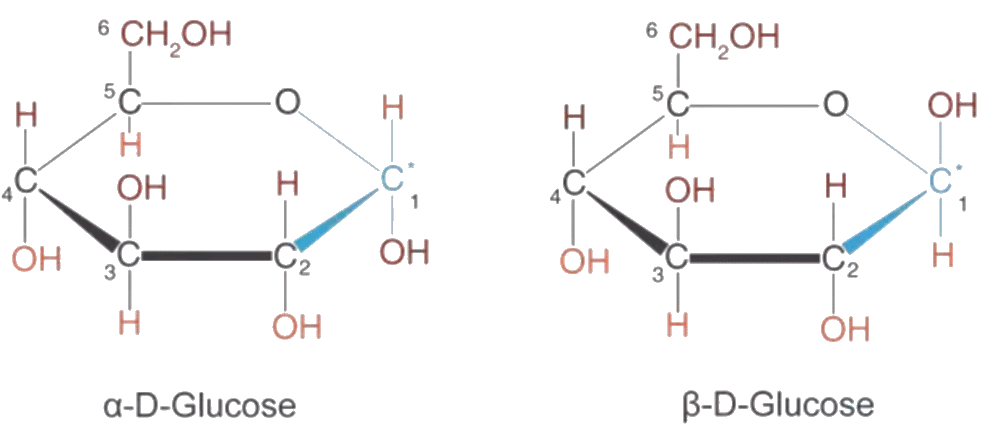
\includegraphics[width=0.6\linewidth]{A2.png}\end{center}
    \item \textit{Galactose} is similar to glucose, but has the $OH$ flipped on carbon-4.
    \item \textit{Fructose}, while it might not seem like it, is also an isomer of glucose:
    \begin{center}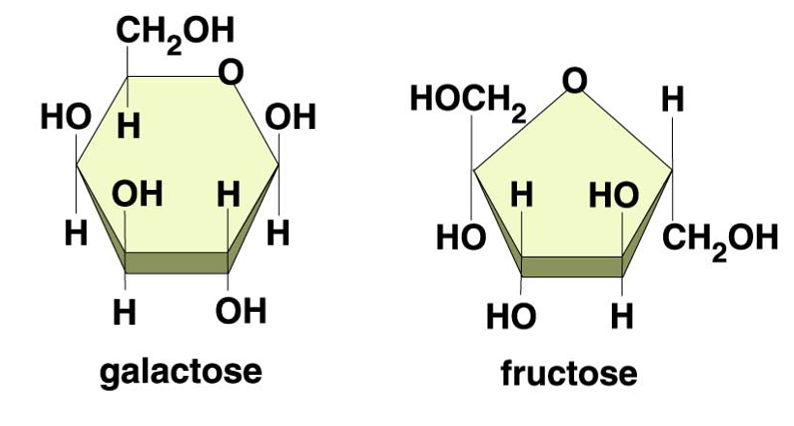
\includegraphics[width=0.6\linewidth]{A4.png}\end{center}
    While the carbons in galactose and glucose are numbered clockwise from the rightmost carbon, fructose has \textit{carbon 2} as the leftmost carbon.

    \item \textbf{Disaccharides} are also simple carbohydrates composed of two sugar units formed from a dehydration reaction.
    
    \begin{itemize}
        \item The linkage is called an \textit{a-b glycosidic linkage} where $a$ and $b$ refer to the carbon that is bonding.
    \end{itemize}
    \begin{idea}
        There are three disaccharides:
        % \begin{multicols}{2}
        \begin{itemize}
            \item Sucrose = Glucose + Fructose (table sugar)
            \item Lactose = Glucose + Galactose (milk)
            \item Maltose = Glucose + Glucose (seed sugar)
        \end{itemize}
        % \end{multicols}
        Many of these are created from a dehydration reaction between monosaccharides.
        \end{idea}
    \item If you used one alpha-glucose on the left, and one beta-glucose on the right, you would end up with a maltose, called beta-maltose, because the ``free anomeric carbon" (i.e., the carbon 1 on the right side of maltose), is in the beta form.
    \begin{center}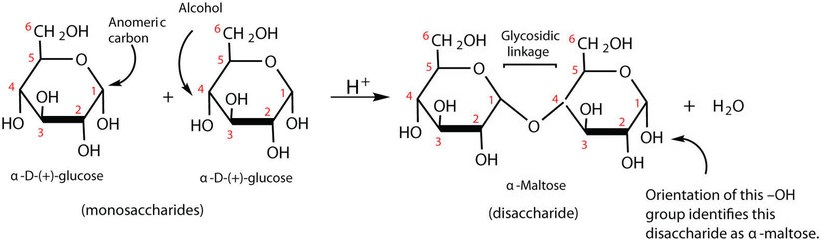
\includegraphics[width=0.8\linewidth]{A1.png}\end{center}
    \begin{idea}
        \textbf{Polysaccharides} have many different sugar units with differing functions:
        % based on chemical makeup and bonding.
        \begin{itemize}
            \item Starch - storage in plants
            \item Glycogen - storage in animals
            \item Cellulose - plant cell walls (strong structure), indigestible
            \item Chitin - exoskeleton of insects (strong structure), fungal cell walls
        \end{itemize}
    \end{idea}
    \item If you join two beta-glucoses together you form the \textbf{disaccharide cellobiose}, and it is linked via a \textit{beta-1,4-glycosidic} bond. If you continue this process to make a polysaccharide, you end up with the cellulose. There can be as many as $10,000$ glucose molecules in a single chain.
    \begin{center}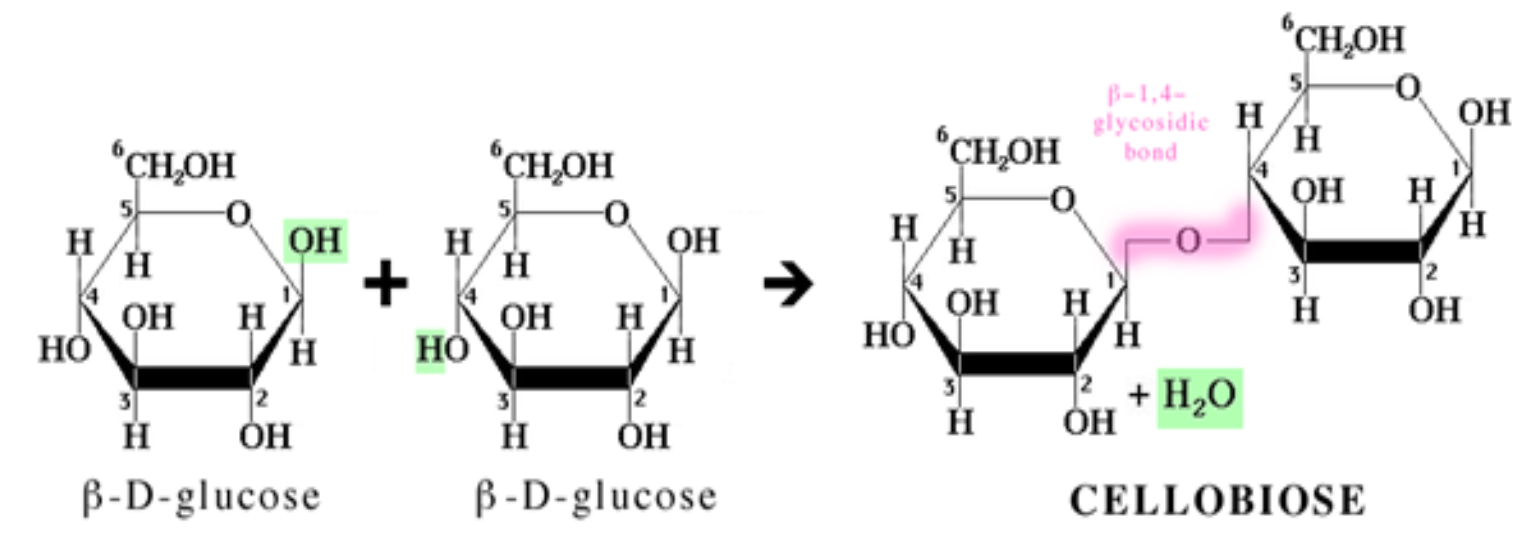
\includegraphics[width=0.8\linewidth]{A3.PNG}\end{center}
    \item \textbf{Cellulose} has a $1,4$ linkage of $\beta$ glucose monomers, creating a zigzag pattern. This makes it harder to digest. Parallel chains become cross-linked with hydrogen bonds and form bundles of $60-70$ molecules called \textbf{microfibrils}, making it very strong and thus are an asset to cell walls.
    \item \textbf{Starch} has a $1,4$ linkage of $\alpha$ glucose monomers, meaning the oxygens are all on the same side, and is easier to digest.
    \begin{itemize}
        \item $30\%$ is \textbf{amylose} which is an unbranched chain linked by $\alpha-1,4$ glycosidic bonds.
        \item $70\%$ is \textbf{amylopectin}, which is a branched chain with $\alpha-1,6$ glycosidic bonds mixed in with $\alpha-1,4$ bonds.
    \end{itemize}
    \item \textbf{Glycogen} is chemically similar to amylopectin, but has more $\alpha-1,6\%$ bonds making it branched more and more water-soluble. It is readily hydrolyzed by enzymes to frm glucose.
    \item \textbf{Chitin} is made of $\beta$-glucose molecules that are chemically similar to cellulose but each glucose has an amine group attached. After cellulose, chitin is the second most abundant carbohydrate.
    \begin{review}
        % \begin{minipage}
        % \begin{table}[]
            \begin{tabular}{lllll}
                \hline
                 & \textbf{Starch} & \textbf{Glycogen} & \textbf{Cellulose} & \textbf{Chitin} \\ \hline
                Monomer & $\alpha$ glucose & $\alpha$ glucose & $\beta$ glucose & $\beta$ glucose \\ \hline
                Linkage & \begin{tabular}[c]{@{}l@{}}1,4 OR\\ 1,6 / 1,4\end{tabular} & 1,4 / 1,6 & 1,4 & 1,4 \\ \hline
                Shape & \begin{tabular}[c]{@{}l@{}}linear / coils OR\\ branched\end{tabular} & \begin{tabular}[c]{@{}l@{}}branched \\ and compact\end{tabular} & \begin{tabular}[c]{@{}l@{}}parallel\\ linear chains\end{tabular} & \begin{tabular}[c]{@{}l@{}}stronger \\ linear chains\end{tabular} \\ \hline
                Function & plant energy storage & \begin{tabular}[c]{@{}l@{}}animal energy\\ storage\end{tabular} & plant cell wall & insect skeleton \\ \hline
                Other & \begin{tabular}[c]{@{}l@{}}soluble OR\\ insoluble\end{tabular} & soluble & hydrophilic & insoluble \\ \hline
                \end{tabular}
        % \end{table}
        % \end{minipage}
    \end{review}

    \begin{lab}
        \textbf{Benedict's} solution is a chemical reagent used to detect the presence of reducing sugars, which have free ketone or aldehyde functional groups. When Benedict’s solution and simple carbohydrates are heated, the solution changes to orange red/ brick red. This reaction is caused by the reducing property of simple carbohydrates. The copper (II) ions in the Benedict’s solution are reduced to Copper (I) ions, which causes the color change. \\

        As a result, this can be used to determine the ripeness of bananas and other fruits as in the presence of air, starch breaks down into glucose which is a reducing sugar that can be tested. \\

        The \textbf{iodine test} is used to test for the presence of starch. Starch turns into an intense "blue-black" colour upon addition of iodine. In the absence of starch, the brown colour of the aqueous solution remains.
    \end{lab}
    \subsection{Lipids}
    \begin{idea}
        Lipids are hydrophobic macromolecules that are separated into four groups:
        \begin{multicols}{2}
            \begin{itemize}
                \item Fats and Oils
                \item Phospholipids
                \item Waxes
                \item Steroids
            \end{itemize}
        \end{multicols}
        They have many functions, which include:
        \begin{itemize}
            \item Fats act as a concentrated energy source.
            \item Phospholipids and cholesterol act as structural components of cell membranes.
            \item Steroid hormones are useful for communication.
            \item Waxes create protection from water.
        \end{itemize}
    \end{idea}
    \item Fats and oils are known as \textbf{triglycerides}. They provide long term energy storage and contain twice the energy as carbohydrates. They also protect internal organs and insulate the body. \textit{They are composed of:} 1 glycerol molecule and 3 fatty acid molecules.
    \item \textbf{Fatty acid} chains are attached to a glycerol molecule and can be \textit{saturated} or \textit{unsaturated}.
    \item Saturated fatty acids is a linear molecule (recall carboxylic acids in \ref{sec:carboxylic}) with no double bonds between carbons. It is solid at room temperature and unhealthy.
    \begin{itemize}
        \item Mammals and birds are more likely than other animals to store energy as saturated fat because of their high body temperatures.
    \end{itemize}
    \item Unsaturated fatty acids contain \textit{at least} one double bond between carbons. This causes the molecule to bend and become liquid at room temperature. It is found in plants and is healthy.
    \begin{multicols}{2}
    \begin{itemize}
        \item Monounsaturated: $1$ double bond
        \item Polyunsaturated: $>1$ double bond
    \end{itemize}
    \end{multicols}
    \item They are attached to a \textbf{glycerol} molecule (\textit{Propane-1,2,3-triol}) through three ester linkages.
    \begin{center}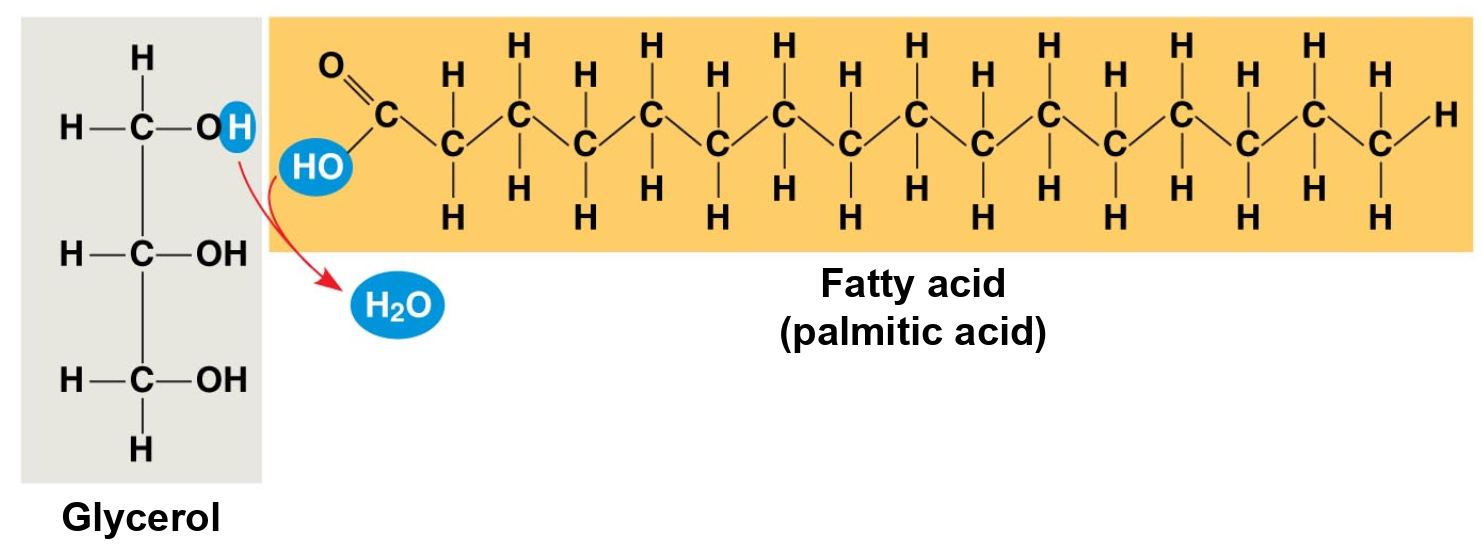
\includegraphics[width=0.6\linewidth]{A6.PNG}\end{center}
    \item \textbf{Phospholipids} are the main component of cell membranes. \textit{It is composed of:} glycerol, 2 fatty acid chains (insoluble), phosphate group in a polar head (soluble). Is is connected via phosphate esters:
    \begin{center}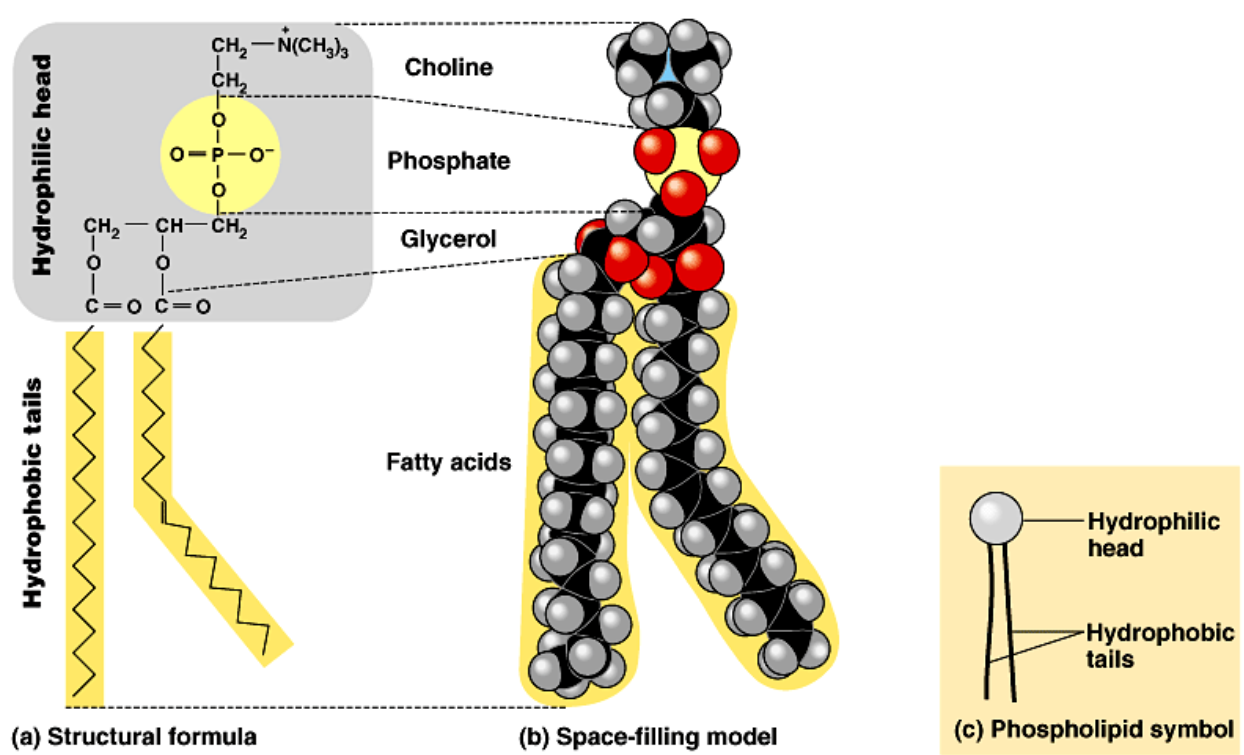
\includegraphics[width=0.6\linewidth]{A7.PNG}\end{center}
    Because of their bilayer nature, they are able to be organized to become a major component of the cell membrane.
    \item \textbf{Waxes} are composed of long fatty acid chains attached
    to alcohol or carbon rings. Since they are hydrophobic, they are used as waterproof protection on plants and animals. They have several purposes:
    \begin{itemize}
        \item Birds have wax that keep their feathers dry.
        \item Plants have a type of wax called \textbf{cutin} that is produced by certain plant cells to form a water-resistant coating on the surfaces of stems, leaves, and fruit. It enables plants to conserve water, and it acts as a barrier to infections and diseases.
        \item Beses use wax to make their honey combs.
    \end{itemize}
    \item \textbf{Steroids} have four linked carbon rings:
    \begin{center}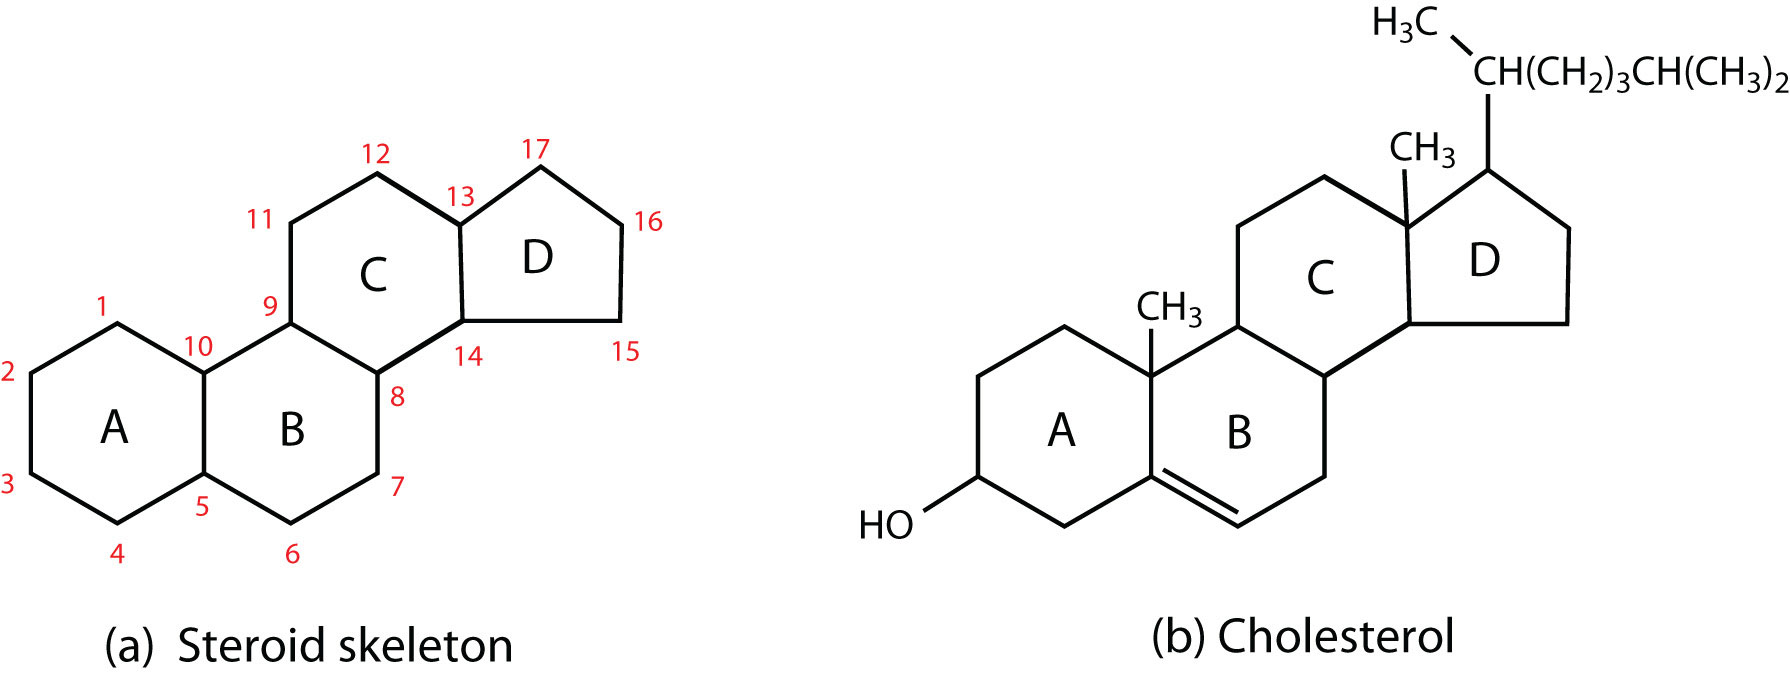
\includegraphics[width=0.7\linewidth]{A8.jpg}\end{center}
    \textit{We are expected only need to be able to recognize them} 
    \item The most abundant steroids, the \textbf{sterols}, have a single polar $-OH$ group at one end of the ring framework and a complex, non-polar hydrocarbon chain at the other end. Although sterols are almost completely hydrophobic, the single hydroxyl group gives one end a \textit{slightly polar, hydrophilic character}. As a result, sterols also have dual solubility properties and, like phospholipids, tend to assume positions in cells that satisfy these properties.
    \item \textbf{Cholesterol} is a sterol that is essential for animal cell membranes and converts into a number of compounds, such as vitamin D. It is an important component of the plasma membrane that surrounds animal cells
    \item \textbf{Phytosterols} is a sterol that performs the same function as cholesterol, but for plants.
    \subsection{Proteins}
    \item Proteins are found in keratin, collagen, chaperons, enzymes, hemoglobin.
    \begin{idea}
        Proteins are a major part as 50\% of our biomass is protein. They are built from amino acid chains. The R-groups play a significant role by bonding with other molecules and give the names for the amino acids. There are three categories of amino acids which are based off their R-group:
        \begin{multicols}{3}
        \begin{itemize}
            \item Nonpolar
            \item Polar
            \item Electrically Charged
        \end{itemize}
        \end{multicols}
    \end{idea}
    \item When two amino acids bond together, they are known as a \textbf{dipeptide}. Their peptide bond can actually interact with other peptide bonds. \textbf{Polypeptides} are created by linking multiply amino acids together.
    \item There are \textit{four different levels} of a protein structure: primary, secondary, tertiary, quaternary.
    \item The \textbf{primary} structure has no functionality, and is only a long chain of amino acids. The ordering of this amino acid is dictated by the DNA, known as \textit{protein synthesis}.
    \item The \textbf{secondary} structure can fold the chain to three different shapes:
    \begin{multicols}{3}
    \begin{itemize}
        \item $\alpha$ Helix
        \item $\beta$ pleated sheet
        \item random coil
    \end{itemize}
    \end{multicols}
    \item The \textit{glue} that holds the secondary structure in this shape through hydrogen bonds with a double bond between the oxygen from the aldehyde group with the hydrogen from the amine group. These bonds are shown with dots.
    \item The \textbf{tertiary} structure is a further folded structure due to attractions and repulsions \textit{between the R groups}. As a result, any bond can be formed within the protein.
    \begin{itemize}
        \item The strongest of which is the \textbf{disulfide bridge}.
    \end{itemize}
    \item The \textbf{quaternary} structure contains multiple polypeptide chains.
    \item If proteins are exposed to very high heat, proteins can be denatured such that their proteins "unravel."
    \begin{center}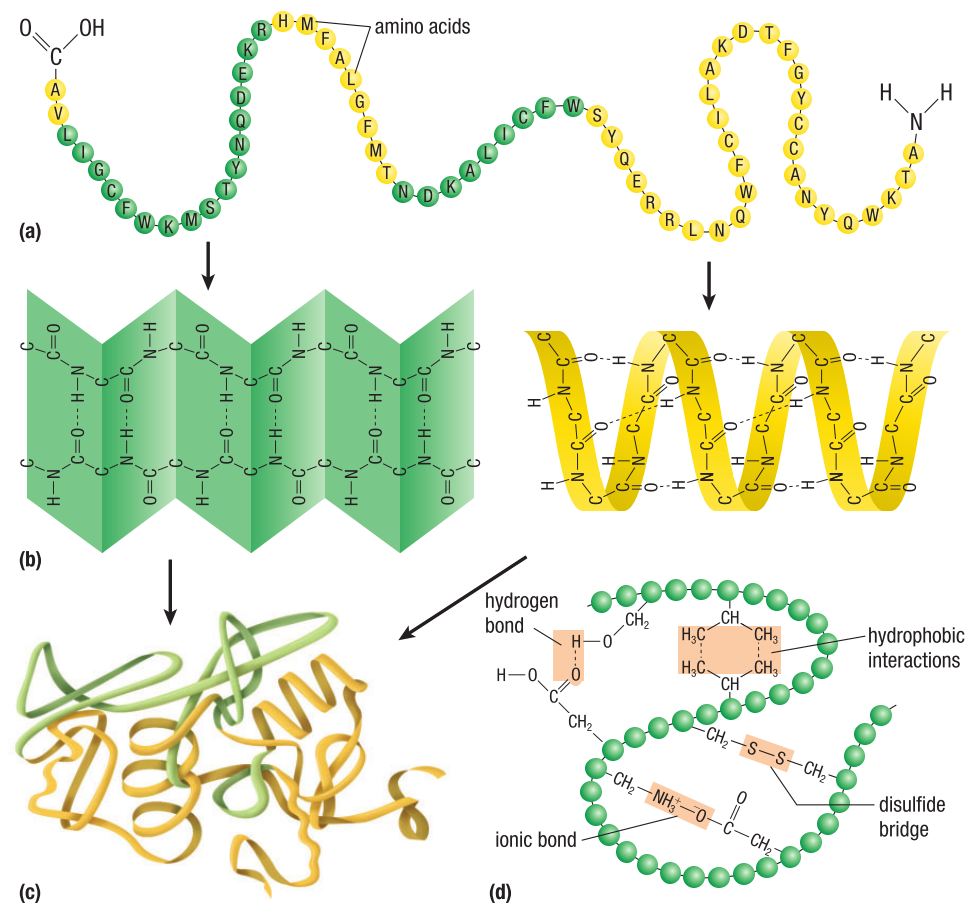
\includegraphics[width=0.75\linewidth]{A9.PNG}\end{center}
    \item The \textbf{nitrogen cycle} helps build the proteins as it is a major part of creating the amines needed to create amino acids.

    \subsection{Nucleic Acids}
    \begin{idea}
        Polymers made from monomers called \textbf{nucleotides}. The three parts of a nucleotide are:
        \begin{itemize}
            \item a phosphate group
            \item a 5 carbon sugar
            \item one of four nitrogenous bases
        \end{itemize}
    \end{idea}
    \item Alternating sugar and phosphate subunits bond to form the "backbone" of a DNA or RNA molecule. \textit{Nitrogenous} bases point inwards like rungs on a ladder
    \item There are three types of nucleic acids: DNA, RNA, ATP
    \item \textbf{Deoxyribonucleic Acid} contains the genetic code for all inheritab le characteristics.
    \item \textbf{Ribonucleic Acid} encodes information necessary for the formation of proteins
    \item \textbf{Adenosine Triphosphate} is an energy carrier made in mitochondria and is produced during the breakdown of glucose.
\end{itemize}
\newpage
\section{Cell Structure}
\begin{itemize}
    \item Emergent properties emerge from macromolecules working together to create cell oraganelles.
    \subsection{The Nucleus}
    \item A \textbf{nuclear envelope} a two lipid bilayer membrane that encloses the nucleus of a eukaryotic cell. The outer bilayer of the membrane is continuous with the endoplasmic reticulum.
    \item This membrane is \textit{selectively} permeable, with active and passive transport systems. Various molecules that access DNA may need to cross through this membrane so this control is a safety mechanism to protect DNA and regulate production of RNA.
    \item The nucleus contains at least one \textbf{nucleolus}, a dense irregularly shaped region where subunits of ribosomes are assembled from proteins and RNA.
    \begin{center}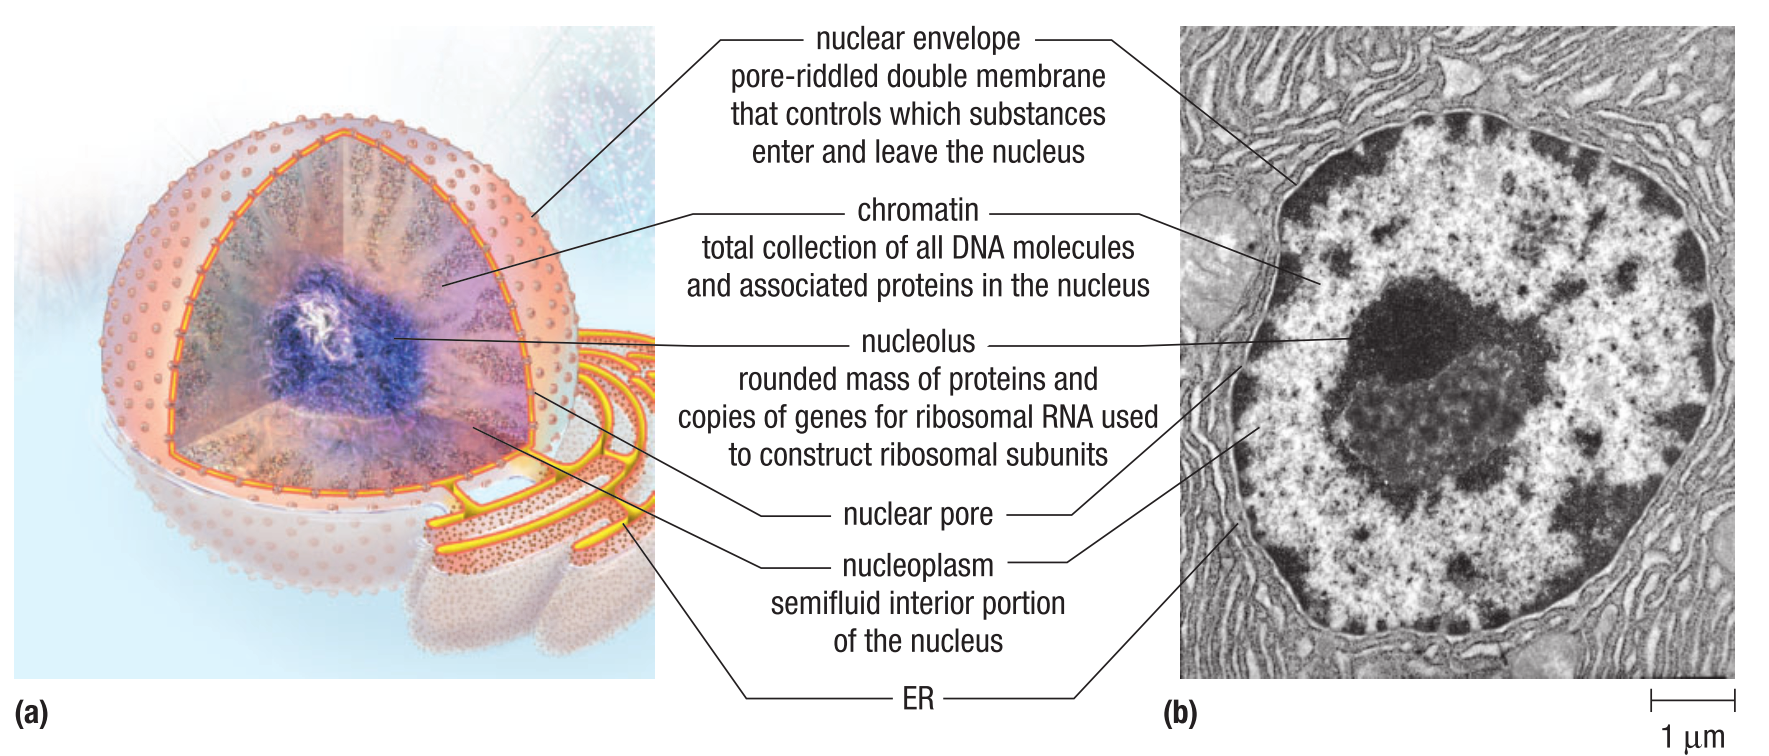
\includegraphics[width=0.9\linewidth]{A10.PNG}\end{center}
    \subsection{Endomembrane System}
    \item The endomembrane system is a group of interacting organelles between the nucleus and the plasma membrane.
    \begin{itemize}
        \item \textit{Purpose: } Make lipids, enzymes, proteins, for secretion or insertion into cell membranes. It also has other specialized functions, such as destroying toxins and recycling wastes.
    \end{itemize}
    \item The \textbf{endoplasmic reticulum} is an extension of the nuclear envelope that forms a continuous compartment that folds repeatedly into flattened sacs and tubes.
    \begin{itemize}
        \item Rough ER - areas of endoplasmic reticulum with ribosomes attached to the surface. Proteins fold and take on complex structures. Some become part of the ER membrane itself, whereas other are carried to different destinations. Cells that make, store, and secrete a lot of proteins have a lot of rough ER.
        \item Smooth ER - areas of the endoplasmic reticulum without attached ribosomes. Some polypeptides made in the rough ER end up in smooth ER as enzymes. These enzymes produce most of the cell’s membrane lipids. They also break down carbohydrates and fatty acids.
    \end{itemize}
    \item \textbf{Vesicles} are saclike membrane-enclosed organelles. They transport proteins from one organelle to another, or to and from the plasma membrane.
    \item \textbf{Peroxisome} is a type of vesicle that contains enzymes that digest fatty acids and amino acids. They form and divide on their own and have a variety of functions, such as inactivating hydrogen peroxide, a toxic by-product of fatty acid breakdown.
    \item A \textbf{Vacuole} is another type of vesicle that stores waste and aids in cellular metabolism and water balance. In \textit{plants}, a large central vacuole is present. Amino acids, sugars, ions, wastes, and toxins accumulate in the water-filled interior. Fluid pressure in the central vacuole keeps the plant cell firm.
    \item \textbf{Lysosomes} are vesicles that contain powerful digestive enzymes. They fuse with vacuoles that carry particles or molecules for disposal, such as worn-out cell components.
    \item Many vesicles fuse with and empty their contents into a \textbf{Golgi body} . This organelle has a folded membrane. Enzymes in a Golgi body put finishing touches on polypeptide chains and lipids that have been delivered from the ER.
    \begin{review}
        There are six steps in building lipids and many proteins as they are transported to other cellular destinations:
        \begin{enumerate}
            \item Inside the nucleus, DNA instructions for making proteins are transcribed into RNA, which moves through nuclear pores into the cytosol.
            \item Some of the RNA in the cytosol is translated into polypeptide chains by ribosomes on the rough ER. The chains enter the rough ER, where they are modified into final form
            \item Vesicles that bud from the rough ER carry some of the new
            proteins to Golgi bodies. Other proteins migrate through the interior of the rough ER and end up in the smooth ER.
            \item Some proteins from the rough ER are packaged into new vesicles and shipped to the Golgi bodies. Others become enzymes of the ER that assemble lipids or inactivate toxins.
            \item Proteins arriving in vesicles from the ER are modified into final form and sorted. New vesicles carry them to the plasma membrane or to lysosomes
            \item Golgi vesicles fuse with the plasma membrane. Lipids and proteins of a vesicle's membrane fuse with the plasma membrane, and the vesicle’s contents are released to the exterior of the cell.
        \end{enumerate}
    \end{review}
    \subsection{Other Organelles}
    \item The \textbf{Cytoskeleton} is supported by many structures:
    \item A \textbf{microtubule} is a long, hollow cylinder that consists of subunits of the protein tubulin. They form a dynamic scaffolding for many cellular processes.
    \item A \textbf{microfilament} is a fibre that consists primarily of subunits of the protein actin. They strengthen or change the shape of eukaryotic cells.
    \item \textbf{Intermediate filaments} are the most stable part of a cell’s cytoskeleton. They strengthen and maintain cell and tissue structures and are the toughest of the cytoskeleton filaments.
    \begin{center}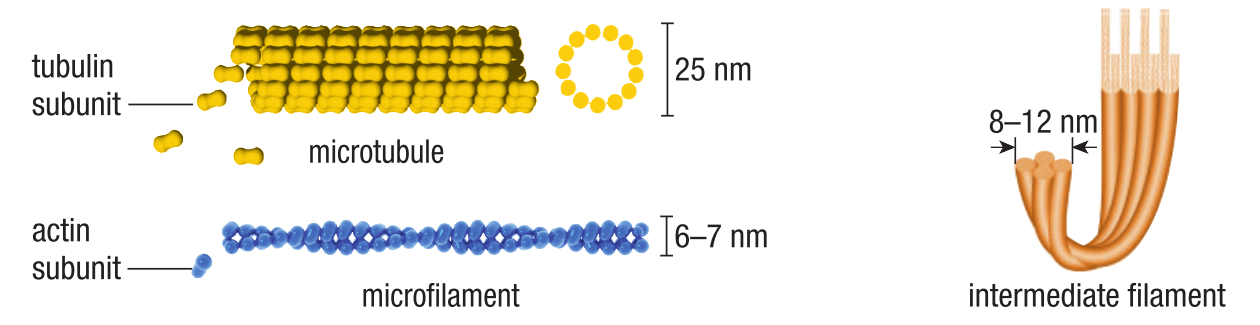
\includegraphics[width=\linewidth]{A11.PNG}\end{center}
    \newpage
    \item The \textbf{Mitochondria} produces large quantities of ATP.
    \begin{itemize}
        \item They have their own DNA, which is similar to bacterial DNA. They divide independently of the cell and have their own ribosomes. Such clues led to the now widely accepted theory of endosymbiosis. According to this theory, mitochondria evolved from aerobic bacteria that took up permanent residence inside a host cell.
    \end{itemize}
    \item \textbf{Plastids} are membrane-enclosed organelles that are used for photosynthesis or storage in plants and algal cells. There are three main types:
    \begin{itemize}
        \item \textbf{Chloroplasts} are double-membrane-bound organelles that contains enzymes and pigments that are used to perform photosynthesis in eukaryotic plant cells.
        \item \textbf{Chromoplasts} are organelles that make and store pigments other than chlorophyll.
        \item \textbf{Amyloplast} are organelles that store starch.
    \end{itemize}
    \item A \textbf{flagella} is a whiplike tail that is used in propulsion of both prokaryotic and eukaryotic cells.
    \item \textbf{Cilia} are tiny hairlike structures that move water and mucus in eukaryotes; used for movement of prokaryotic cells.
    \begin{center}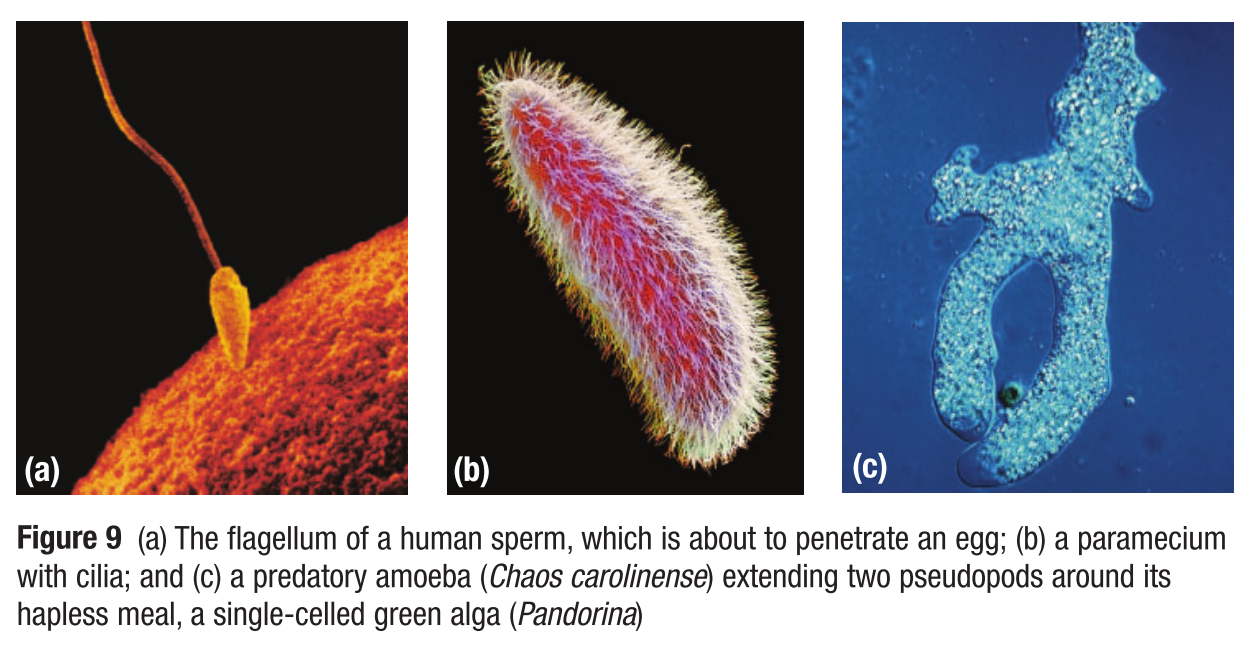
\includegraphics[width=0.6\linewidth]{A12.PNG}\end{center}
    \subsection{Cell Surface}
    \item The \textbf{cell wall} is the outer barrier of a plant cell; it surrounds the plasma membrane and gives structure to the plant.
    \item The \textbf{primary wall} is a cellulose coating that surrounds a plant cell.
    \item However, the \textbf{secondary wall} is a coating that is added to a plant cell wall; it is more rigid and often thicker than the primary cell wall.
    \item An \textbf{extracellular matrix} (ECM) a molecular system that supports and protects a cell; a cell’s environment.
    \begin{center}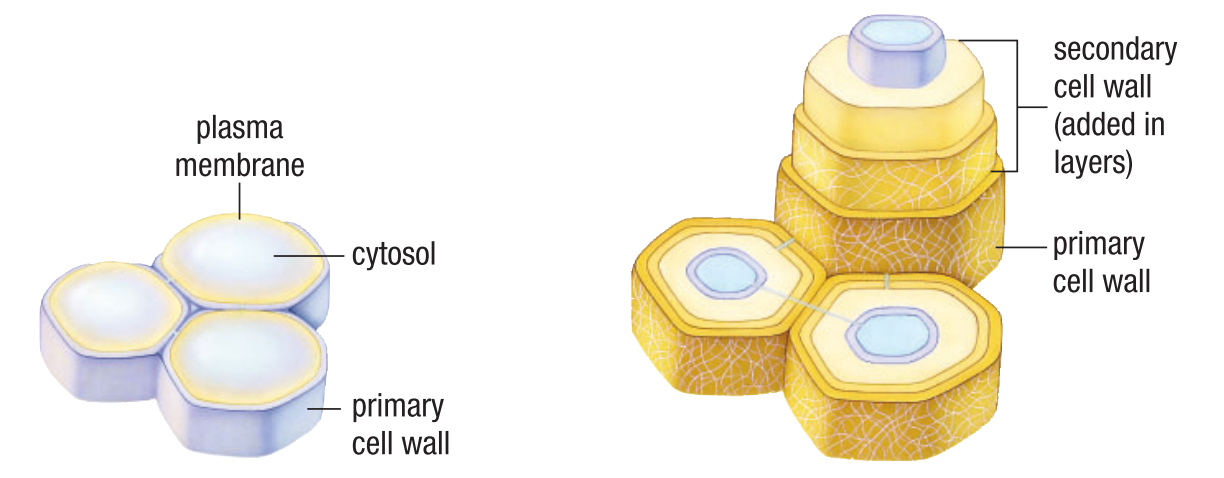
\includegraphics[width=0.6\linewidth]{A13.PNG}\end{center}
\end{itemize}

\newpage
\section{Cell Membrane}
\begin{itemize}
\item Emergent properties emerge around the complexities of the cell membrane with a multitude of macromolecules working together to perform several functions.
\begin{lab}
    The \textbf{Bubble Lab} demonstrated three key features of cell membranes:
    \begin{itemize}
        \item Membranes are fluid and flexible
        \item Membranes can self repair
        \item Membrane proteins perform special functions
    \end{itemize}
\end{lab}
\subsection{Fluid Mosaic Model}
\begin{idea}
    The \textbf{fluid mosaic model} is the idea that a biological membrane consists of a fluid phospholipid bilayer, in which proteins are embedded and float freely.
    \begin{center}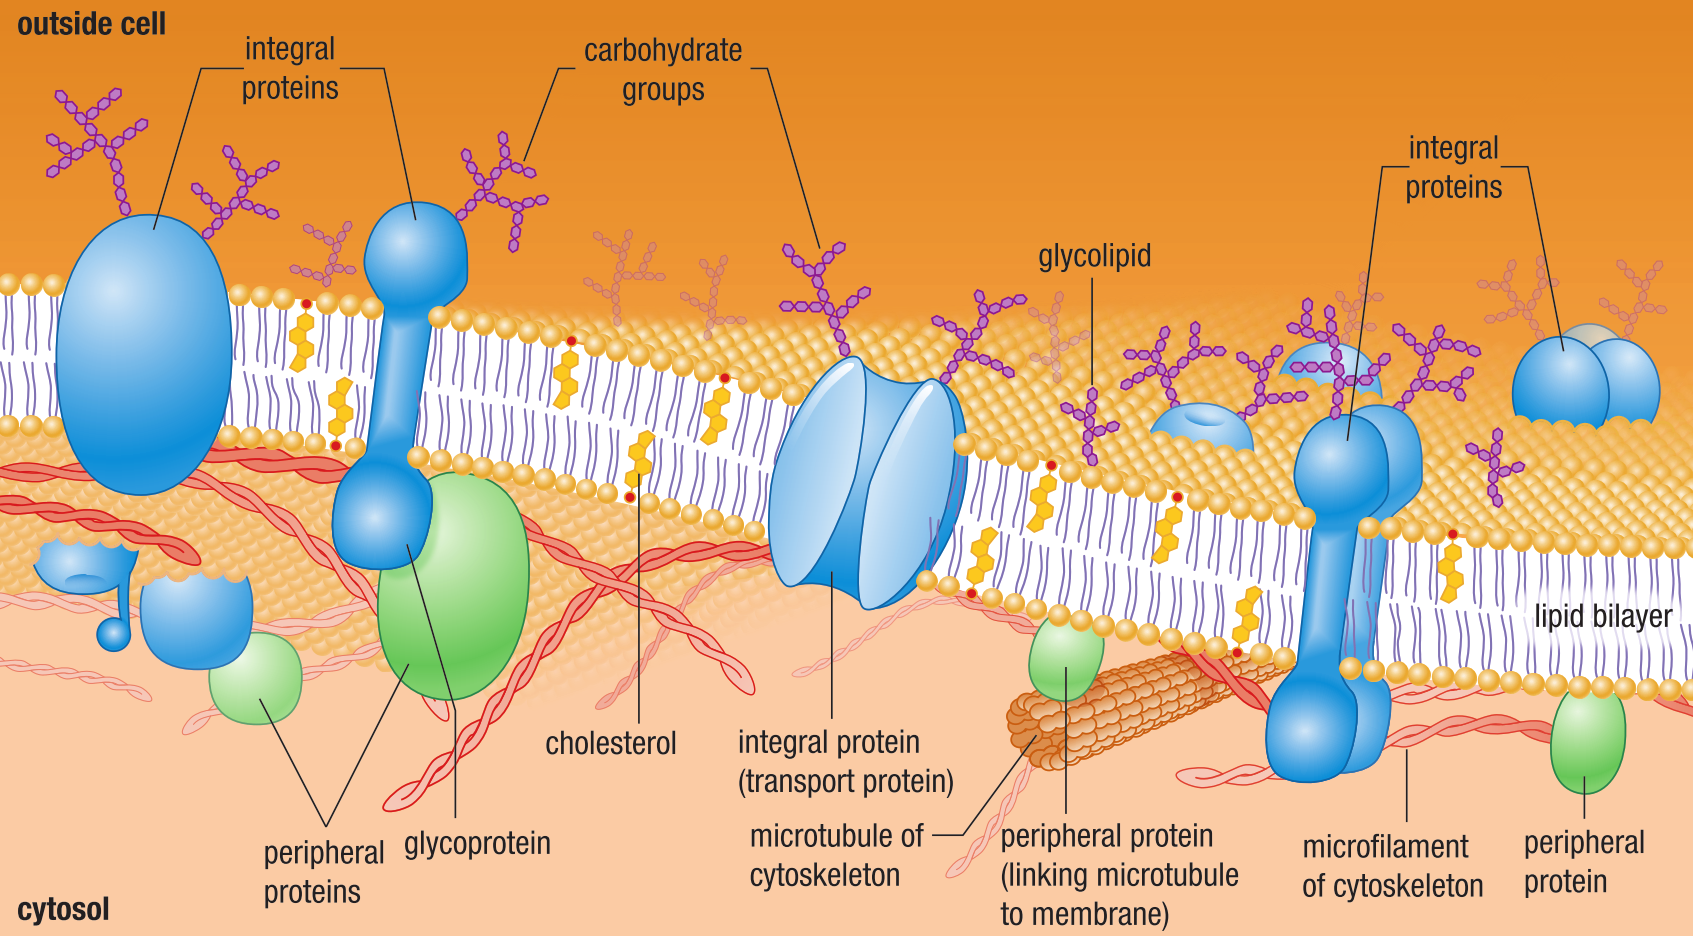
\includegraphics[width=0.9\linewidth]{A14.PNG}\end{center}
    This model proposes that membranes are not rigid, with molecules locked into place.  They are described as a fluid because the lipid and protein molecules are generally free to move laterally within the two layers. Millions of times a second, the lipid molecules may vibrate, flex back and forth, spin around their long axis, move sideways, and exchange places within the same half of the bilayer.
\end{idea}
\item \textbf{glycolipid} and \textbf{glycoproteins} face the exterior of the cell and perform cell-cell communication.
\begin{itemize}
    \item A glycolipid is any membrane lipid that is bound to a carbohydrate
    \item A glycoprotein is a membrane component that contains a sugar, or carbohydrate, bound to an amino acid
\end{itemize}
\item The most important part of the membrane is the phospholipid bilayer. A bilayer forms spontaneously in an aqueous environment because of the tendency of the non-polar hydrophobic fatty acids to aggregate together while the polar heads associate with water.
\item The degree of unsaturated fatty acid tails determines the fluidity of the cell membrane. The more unsaturated a membrane is, the lower its gelling temperature
\begin{itemize}
    \item At the gel point, the system loses fluidity and viscosity becomes very large. The onset of gelation, or gel point, is accompanied by a sudden increase in viscosity.
\end{itemize}
\item Sterols such as cholesterol also affect the fluidity. They help to restrain the movement of the lipid molecules in a membrane, thus reducing the fluidity of the membrane. At lower temperatures, however, sterols occupy the spaces between the lipid molecules, thus preventing fatty acids from associating and forming a non-fluid gel.
\item It is the set of proteins that make the membrane \textit{unique}. Membrane proteins can be separated into four categories:
\begin{itemize}
    \item \textbf{Transport:} a specific compound may be able to cross a membrane by way of a hydrophilic protein channel.
    \item \textbf{Enzymatic Activity:} Some membrane proteins, such as those associated with respiration and photosynthesis, are enzymes.
    \item \textbf{Triggering Signals:} Membrane proteins may bind to specific chemicals, such as hormones. Binding to these chemicals triggers changes on the inner surface of the membrane, starting a cascade of events within the cell.
    \item \textbf{Attachment and Recognition:} roteins that are exposed to both the internal and external membrane surfaces act as attachment points for a range of cytoskeleton elements, as well as components involved in cell–cell recognition, and bond to the extracellular matrix.
\end{itemize}
\begin{center}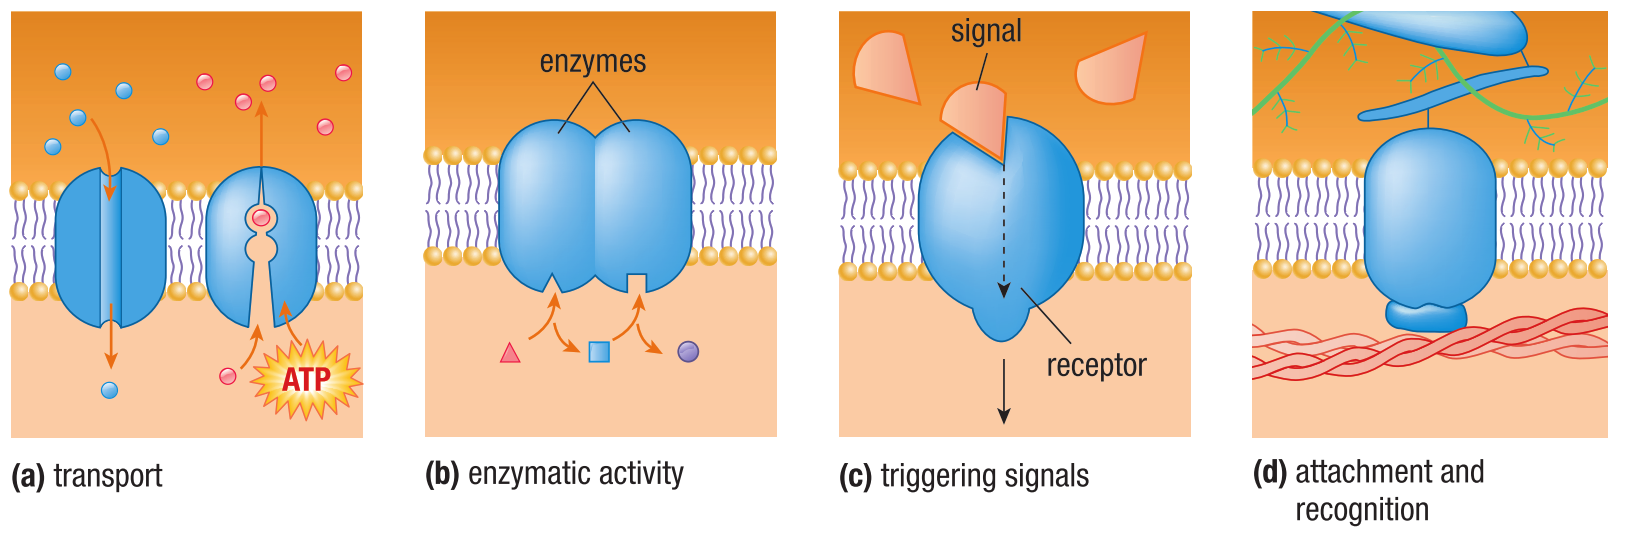
\includegraphics[width=0.9\linewidth]{A15.PNG}\end{center}
\item All of these functions may exist in a single membrane, and one protein or protein complex may serve more than one of these functions. Beyond function, all membrane proteins can be separated into two additional categories: integral and peripheral membrane proteins:
\item An \textbf{integral membrane protein} is a protein that is embedded in the lipid bilayer. Most are transmembrane proteins with a nonpolar part that goes in the middle.
\item A \textbf{peripheral membrane protein} is a protein on the surface of the membrane. Most are on the cytosol portion of the membrane.
\begin{review}
    An important part of the cell membrane is its \textit{asymmetry}. A range of glycolipids and carbohydrate groups attach to proteins on the external half of the membrane, whereas components of the cytoskeleton bind to proteins on the internal half of the membrane. In addition, hormones and growth factors bind to receptor proteins that are found only on the external surface of the plasma membrane. Their binding triggers changes to distinctly different protein components found on the inner surface of the membrane, spurring a cascade of reactions that send signals within the cell.
\end{review}
\begin{lab}
    \textbf{Coacervates}, while not alive, do exhibit some properties in common with living cells. coacervates form a membrane of water around themselves. This membrane acts to control the effects of the external environment on the interior of the coacervate, just as the cell membrane acts. The membrane allows the coacervate to take up and concentrate substances inside of it, increasing it to many times the concentration outside, greatly increasing the rate of reactions within it. It is proposed that as coacervates be become more complex they can carry on more lifelike functions and eventually become heterotrophs and as nutrients decreased, competition allowed them to become even more complex.
\end{lab}
\subsection{Transport}
\begin{idea}
    For a cell to survive and function, it must take in nutrients, expel waste, and communicate with its environment and neighbouring cells. This exchanging of substances is a complex process because the plasma membrane must be highly selective. It must be able to take in very large food molecules while preventing very small and valuable molecules from leaving the cell. It must also be able to recognize foreign substances that are harmful and block their passage while, at the same time, expelling the cell’s toxic waste products. 
\end{idea}
\item \textbf{Passive Transport} is the movement of a substance across a membrane without expending energy. Examples include osmosis and diffusion. When this continued action results in a balanced condition it is known as \textbf{dynamic equilibrium}.
\item The size and charge of a particle affects whether or not it can pass through the membrane.
\begin{center}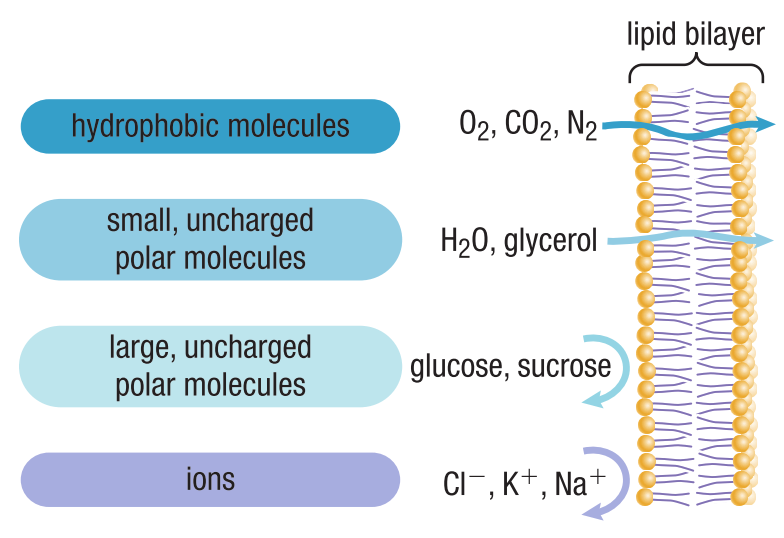
\includegraphics[width=0.4\linewidth]{A16.PNG}\end{center}
\item \textbf{Facilitated diffusion} is the facilitated transport of ions and polar molecules through a membrane via protein complexes. This speeds up the rate of diffusion of some compounds in order to keep up with the demand that metabolic processes often have.
\item Proteins that carry out facilitated diffusion are called \textbf{transport proteins} that extend through the membrane.
\item \textbf{Channel proteins} form hydrophilic pathways in the membrane through which water and certain ions can pass
\begin{center}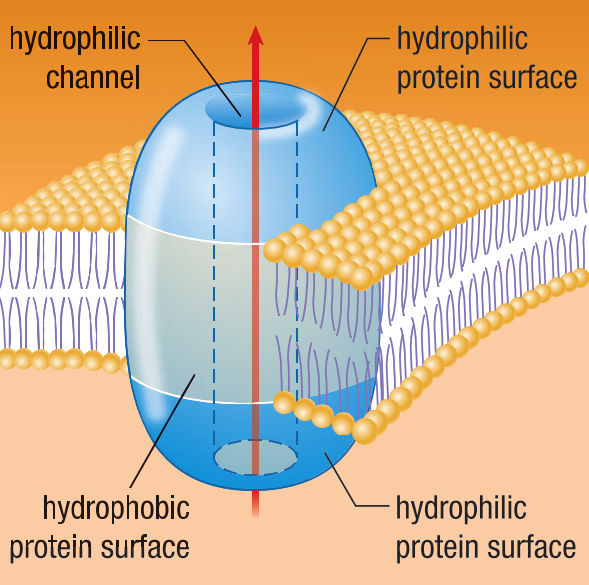
\includegraphics[width=0.4\linewidth]{A17.PNG}\end{center}
\item A \textbf{Carrier Protein} is a protein that binds to a molecule and transports it across the lipid bilayer. Each carrier protein binds to a specific solute, such as a glucose molecule or a particular amino acid, and transports it across the lipid bilayer.
\begin{center}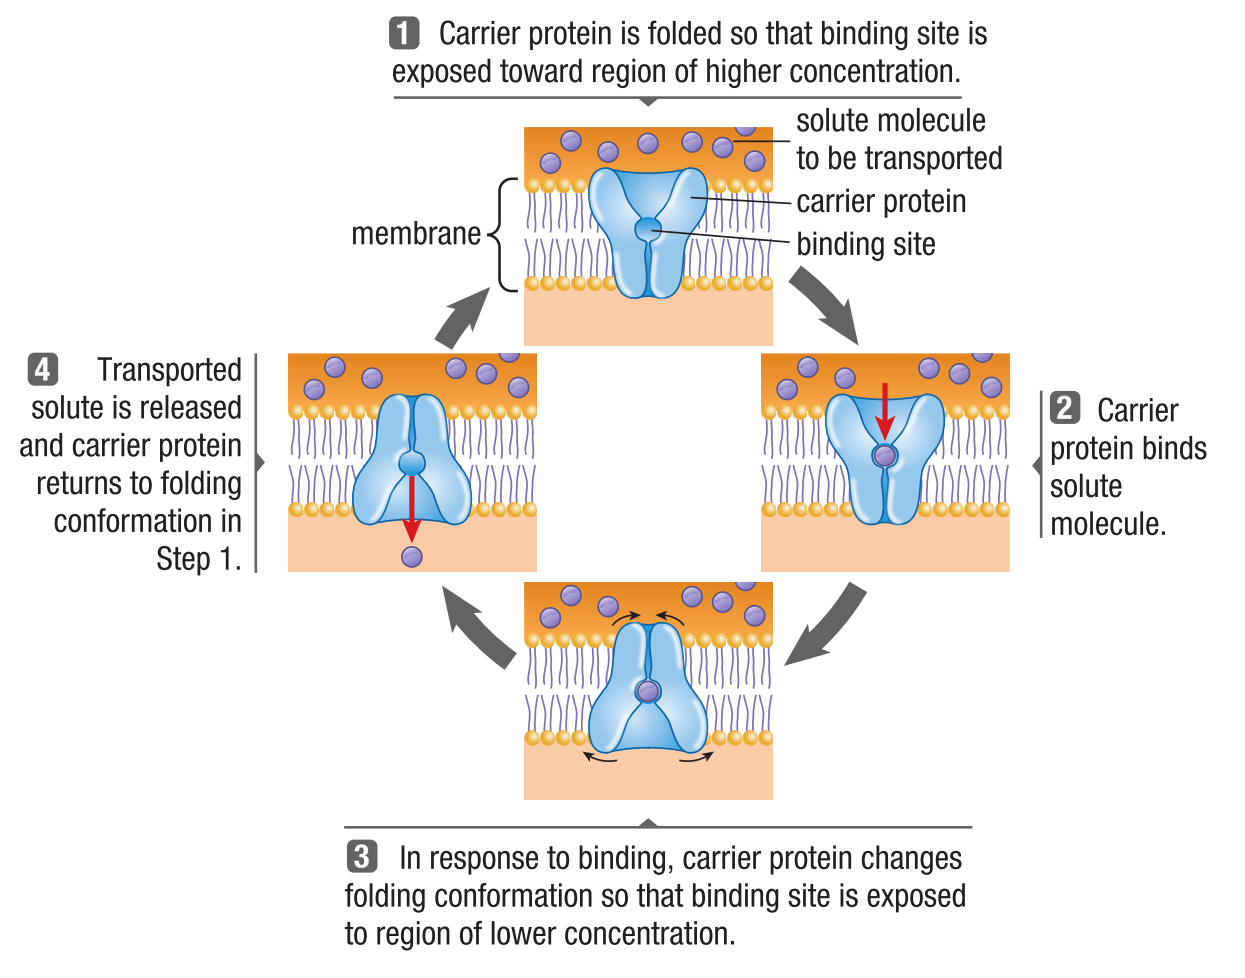
\includegraphics[width=0.8\linewidth]{A18.PNG}\end{center}
although facilitated transport is faster, the maximum rate is quickly reached as it is limited by the number of transport proteins.
\item A solution is \textbf{hypotonic} if it has a lower solute concentration than another solution and it is \textbf{hypertonic} if it has a higher concentration. If both are the same, then they are \textbf{isotonic}.
\item \textbf{Active transport} is the movement of substances across membranes against their concentration gradient using pumps.
\begin{idea}
    Using ``pumps," active transport is able to concentrate specific compounds inside cells and push others out. For example, in muscle cells, the calcium ion concentration in one compartment can be as much as 30 000 times as great as the calcium ion concentration in another compartment. Such a huge concentration difference, which is necessary for normal muscle function, is established and maintained through active transport.
\end{idea}
\begin{center}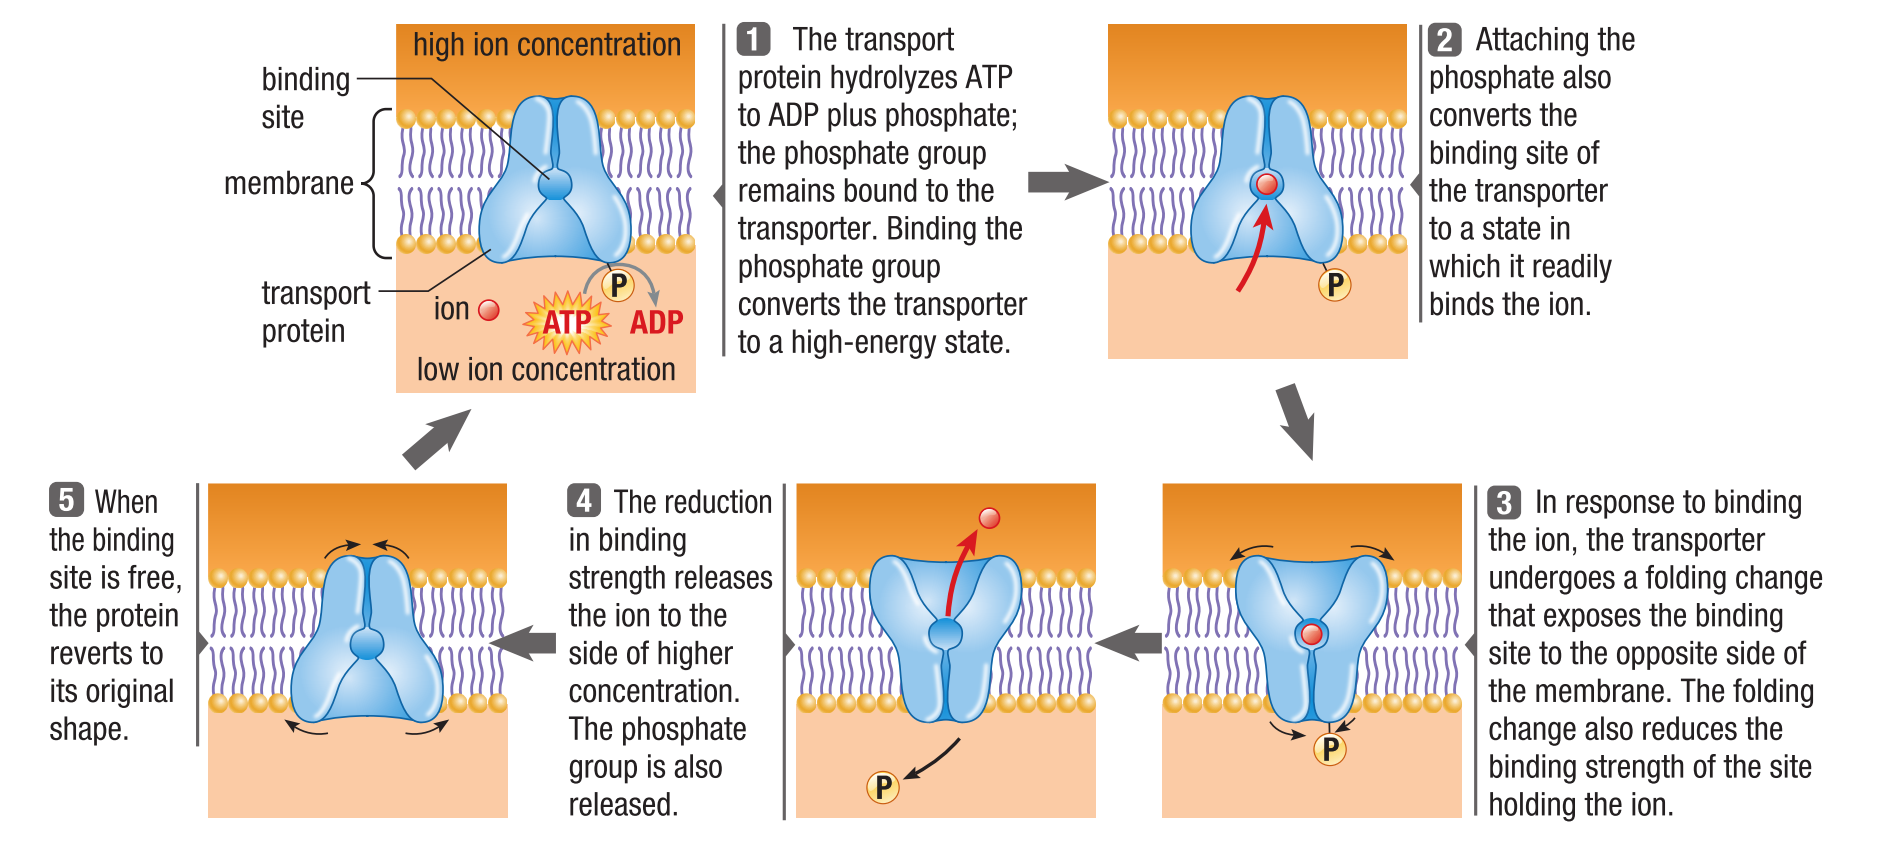
\includegraphics[width=\linewidth]{A19.PNG}\end{center}
\item All primary active transport pumps move positively charged ions across membranes. The concentration gradients that are established by these active transport pumps underlie functions that are absolutely essential for cellular life.
\item An \textbf{electrochemical gradient} is the combined effects of a difference in electrical potential energy and a difference in the concentration gradients of ions.
\item A \textbf{secondary active transport pump} uses the concentration gradient of an ion, established by a primary pump, as its energy source. Secondary active transport is facilitated by two mechanisms, known as \textbf{symport} and \textbf{antiport}:
\begin{itemize}
    \item Symport: the transported solute moves in the same direction as the gradient of the driving ion
    \item Antiport: the transported solute moves in the direction that is opposite to the gradient of the driving ion
\end{itemize}
\begin{center}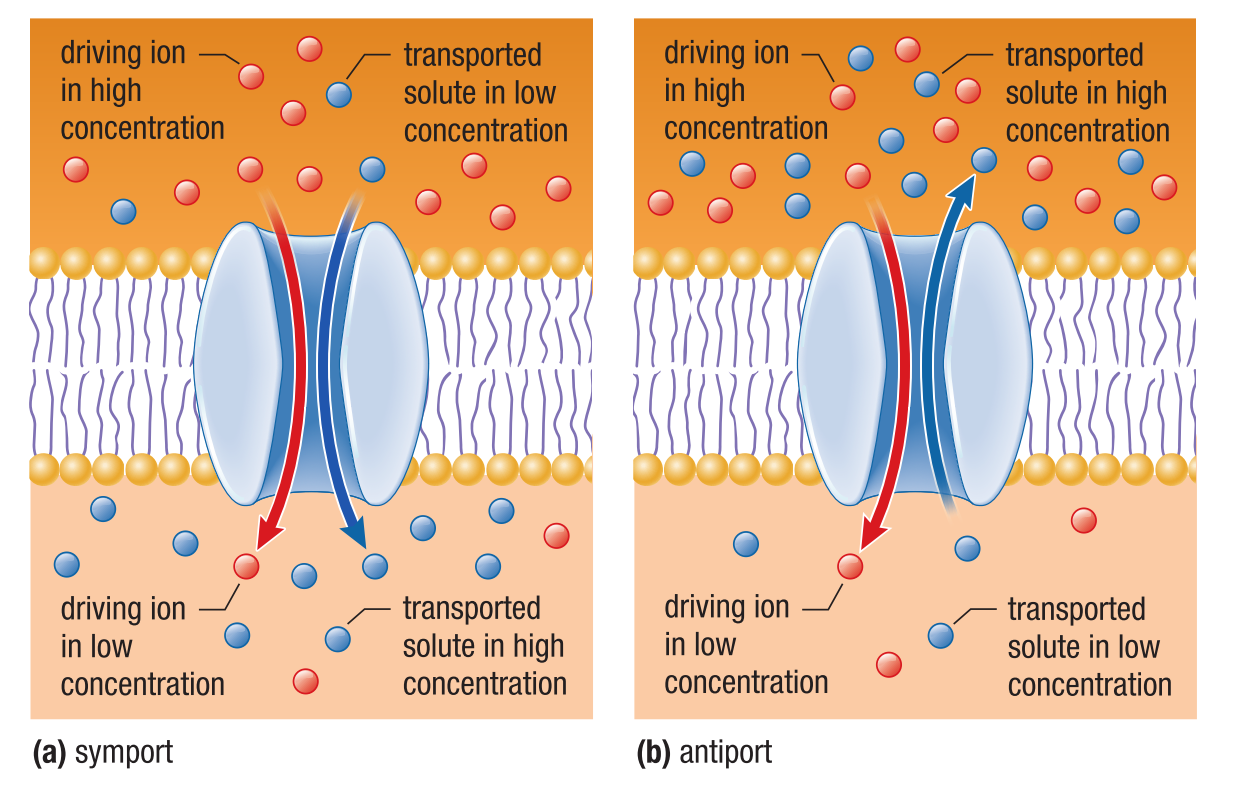
\includegraphics[width=0.6\linewidth]{A20.PNG}\end{center}
\begin{review}
    % \begin{table}[]
        \begin{tabular}{cccc}
        \hline
        \multirow{2}{*}{Characteristic} & \multicolumn{2}{c}{Passive Transport} & \multirow{2}{*}{Active Transport} \\ \cline{2-3}
         & \multicolumn{1}{l}{Simple Diffusion} & \multicolumn{1}{l}{Facilitated Difusion} &  \\ \hline
        \begin{tabular}[c]{@{}c@{}}Membrane component responsible\\ for influencing transport\end{tabular} & lipids & proteins & proteins \\ \hline
        Binding to transported substance & no & yes & yes \\ \hline
        Energy Source & \begin{tabular}[c]{@{}c@{}}concentration\\ gradient\end{tabular} & \begin{tabular}[c]{@{}c@{}}concentration\\ gradient\end{tabular} & \begin{tabular}[c]{@{}c@{}}ATP hydrolysis or \\ concentration\\ gradient\end{tabular} \\ \hline
        Direction of Transport & with gradient & with gradient & against gradient \\ \hline
        Specificity for molecules & non-specific & specific & specific \\ \hline
        \begin{tabular}[c]{@{}c@{}}Saturation at high concentrations\\ of transported molecules\end{tabular} & at & high & concentrations \\ \hline
        \end{tabular}
    % \end{table}
\end{review}
\subsection{Exocytosis and Endocytosis}
\begin{idea}
    The largest molecules that can be transported across a cellular membrane by passive or active transport are about the size of amino acids or monosaccharides such as glucose. However, eukaryotic cells can export and import larger molecules by two other mechanisms, called exocytosis and endocytosis
\end{idea}
\item In \textbf{exocytosis}, secretory vesicles move through the cytosol and contact the plasma membrane. The vesicle membrane fuses with the plasma membrane, releasing the contents of the vesicle to the exterior of the cell.
\begin{center}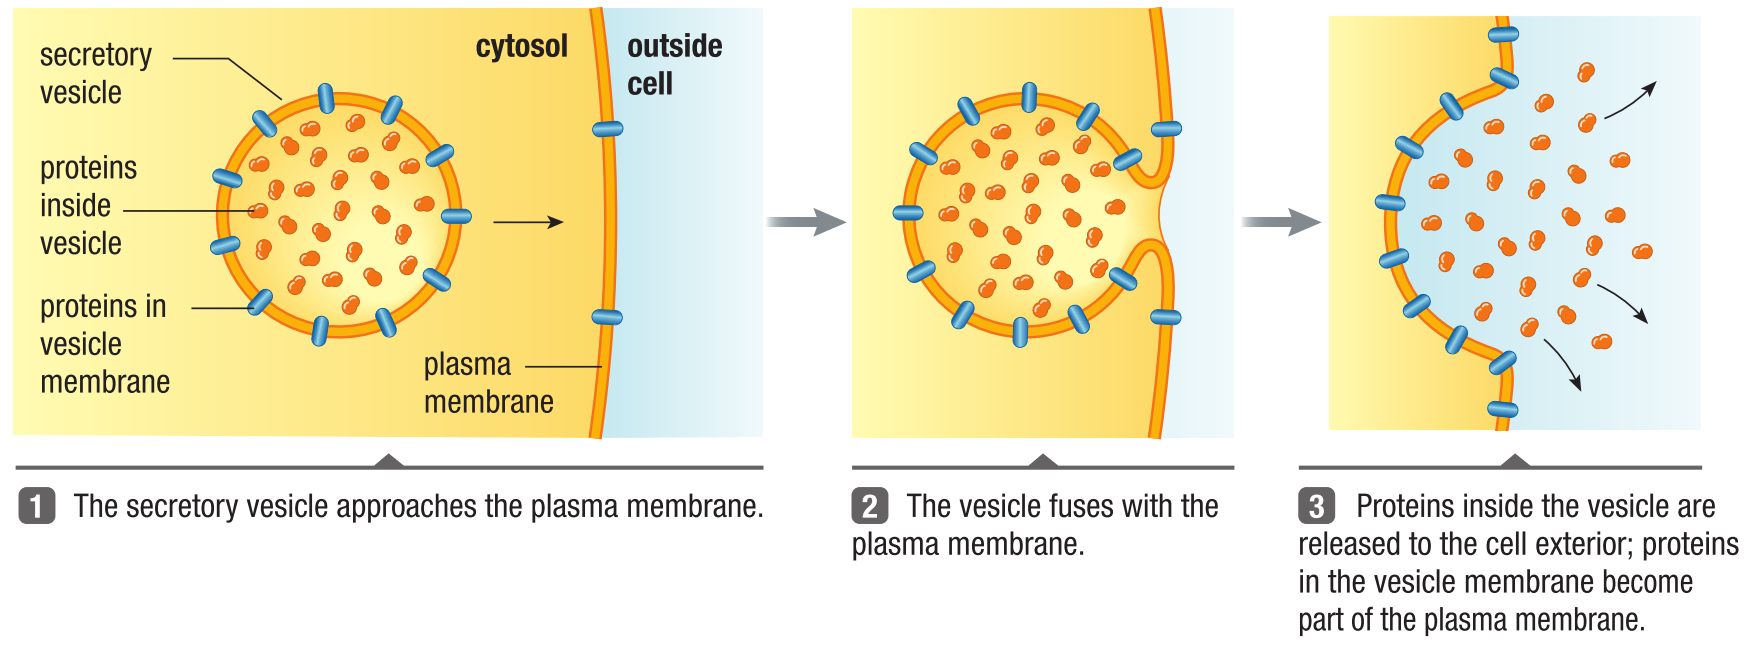
\includegraphics[width=0.8\linewidth]{A21.PNG}\end{center}
\item In \textbf{endocytosis}, proteins and other substances are trapped in a pit-like depression that bulges inward from the plasma membrane. The depression then pinches off as an endocytic vesicle. There are three forms of endocytosis:
\item In \textbf{bulk-phase} endocytosis, or pinocytosis, extracellular water is taken in, along with any molecules that happen to be in solution in the water. No binding by surface receptors takes place.
\begin{center}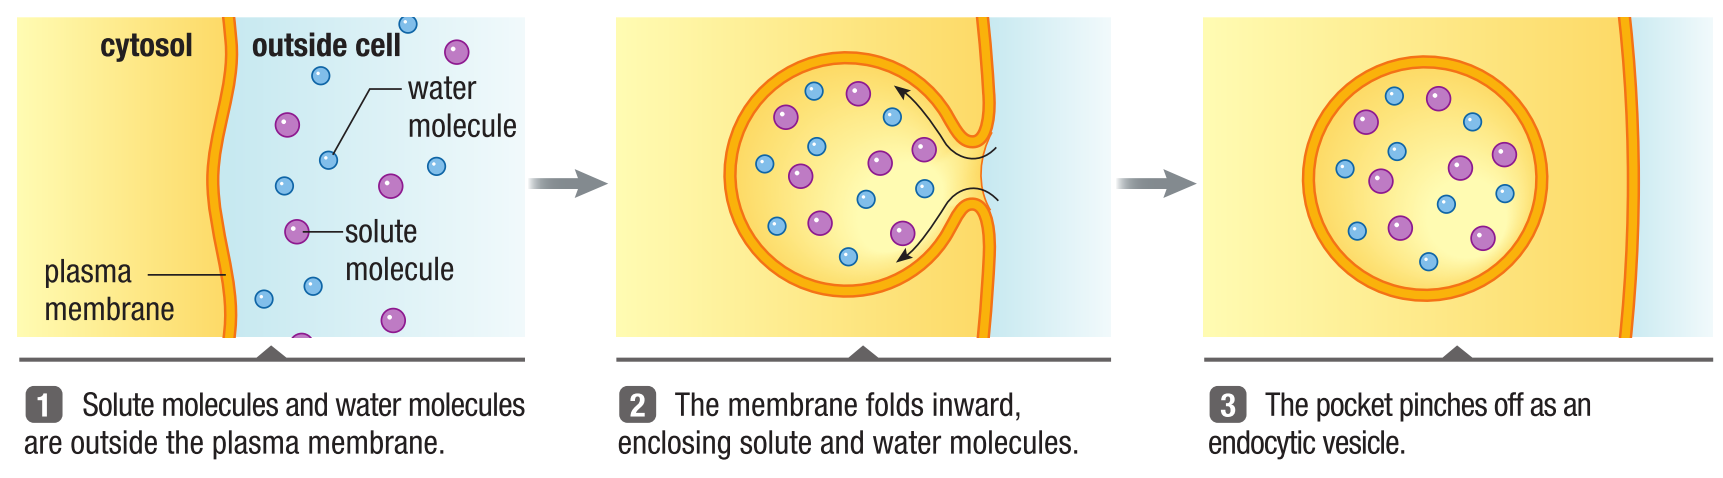
\includegraphics[width=0.8\linewidth]{A22.PNG}\end{center}
\item In \textbf{receptor-mediated} endocytosis, the molecules
to be taken in are bound to the outer cell surface by receptor proteins. The receptors bind to only certain molecules—primarily proteins or molecules carried by proteins.
\begin{center}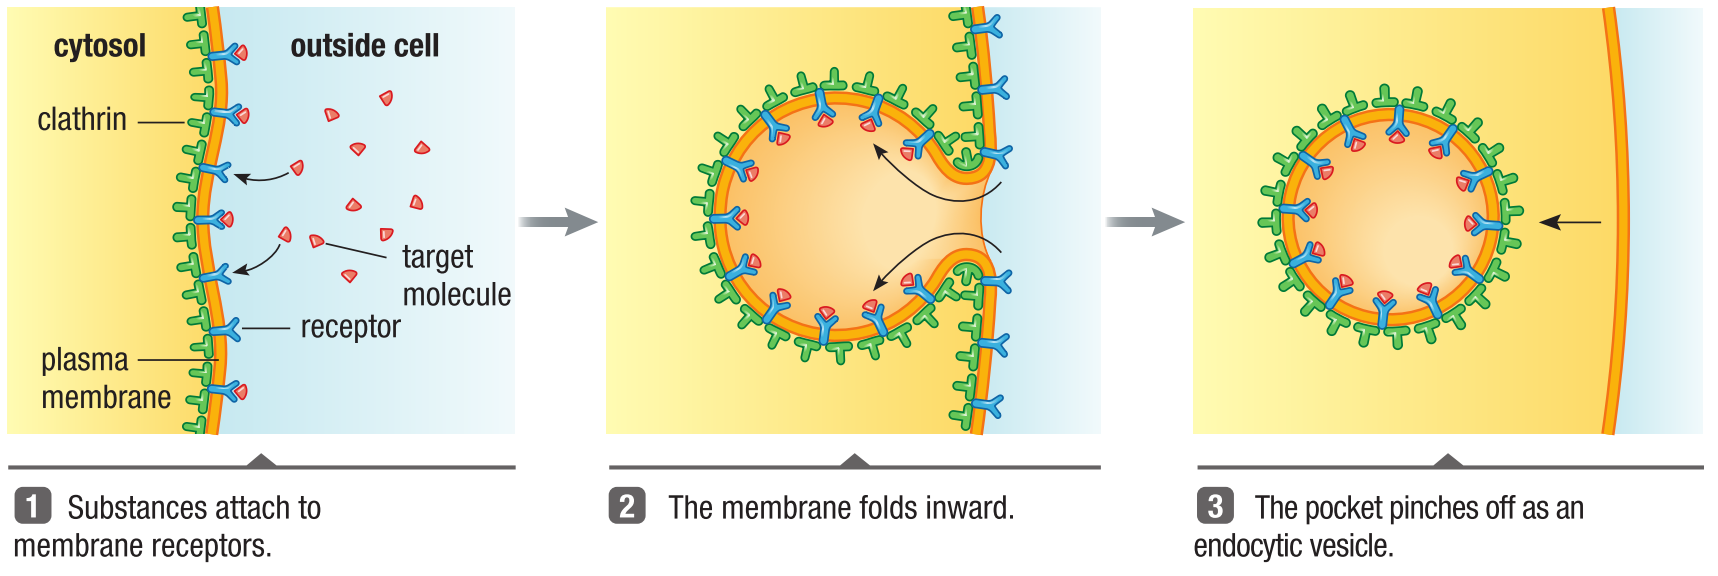
\includegraphics[width=0.8\linewidth]{A23.PNG}\end{center}
After binding, the receptors collect into a pit coated with a network of proteins, called \textbf{clathrin}, that reinforce the cytosol side. The coated pit then breaks free of the membrane to form a vesicle. In the cytosol, the vesicle loses its clathrin coating and may fuse with a lysosome. Enzymes within the lysosome then digest the cargo, breaking it down into smaller molecules that are useful to the cell
\item The third type is \textbf{phagocytosis} where cells engulf bacteria, parts of dead cells, viruses, or other foreign particles. This pathway is most commonly performed by a \textbf{macrophage} like a white blood cell.
\begin{review}
    Through the combined mechanisms of passive transport, active transport, exocytosis, and endocytosis, emergent properties arise. Cells are able to maintain their internal concentrations of ions and molecules and exchange larger molecules, such as proteins, with their surroundings.
\end{review}
\end{itemize}



\end{document}